\documentclass[12pt]{amsart}

%\usepackage{pdfsync}
\usepackage{latexsym,enumitem}
\usepackage{amssymb}
\usepackage[cp850]{inputenc}
\usepackage{epsfig}
\usepackage{psfrag}
\usepackage{amsthm}
\usepackage{amscd}
\usepackage{amsmath}
\usepackage{amsfonts}
\usepackage{graphics,caption}
\usepackage[all]{xy}
\usepackage{etoolbox}
\usepackage{xcolor}
\patchcmd{\quote}{\rightmargin}{\leftmargin 2em \rightmargin}{}{}
\captionsetup{width=4.7in}

\newtheorem{sat}{Theorem}[section]		\newtheorem{lem}[sat]{Lemma}
\newtheorem{kor}[sat]{Corollary}			\newtheorem{prop}[sat]{Proposition}
\newtheorem{bei}{Example}				\newtheorem{defi}[sat]{Definition}
\newtheorem{rmk}[sat]{Remark}
\newtheorem*{defi*}{Definition}			\newtheorem*{bei*}{Example}
\newtheorem*{sat*}{Theorem}				\newtheorem*{kor*}{Corollary}
\newtheorem*{rmk*}{Remark}				\newtheorem{quest}{Question}	
\newtheorem{claim}[sat]{Claim}	
\newtheorem{fact}[sat]{Fact}	

% number equations by section:
\renewcommand{\theequation}{\thesection.\arabic{equation}}
\let\ssection=\section
\renewcommand{\section}{\setcounter{equation}{0}\ssection}

\newtheorem*{namedtheorem}{\theoremname}
\newcommand{\theoremname}{testing}
\newenvironment{named}[1]{\renewcommand{\theoremname}{#1}\begin{namedtheorem}}{\end{namedtheorem}}

\theoremstyle{remark}
\newtheorem*{bem}{Remark}

%\setlength{\parindent}{0em}

%\newcommand{\defin}{\ensuremath{\overset{ \text{\tiny def} }{=} } }

\newcommand{\BC}{\mathbb C}			\newcommand{\BH}{\mathbb H}
\newcommand{\BR}{\mathbb R}			\newcommand{\BD}{\mathbb D}
\newcommand{\BN}{\mathbb N}			\newcommand{\BQ}{\mathbb Q}
\newcommand{\BS}{\mathbb S}			\newcommand{\BZ}{\mathbb Z}
\newcommand{\BF}{\mathbb F}			\newcommand{\BT}{\mathbb T}
\newcommand{\BU}{\mathbb U}
%\newcommand{\RP}{\mathrm P}

\newcommand{\CA}{\mathcal A}		\newcommand{\CB}{\mathcal B}
\newcommand{\CC}{\mathcal C}		\newcommand{\calD}{\mathcal D}
\newcommand{\CE}{\mathcal E}		\newcommand{\CF}{\mathcal F}
\newcommand{\CG}{\mathcal G}		\newcommand{\CH}{\mathcal H}
\newcommand{\CI}{\mathcal I}		\newcommand{\CJ}{\mathcal J}
\newcommand{\CK}{\mathcal K}		\newcommand{\CL}{\mathcal L}
\newcommand{\CM}{\mathcal M}		\newcommand{\CN}{\mathcal N}
\newcommand{\CO}{\mathcal O}		\newcommand{\CP}{\mathcal P}
\newcommand{\CQ}{\mathcal Q}		\newcommand{\CR}{\mathcal R}
\newcommand{\CS}{\mathcal S}		\newcommand{\CT}{\mathcal T}
\newcommand{\CU}{\mathcal U}		\newcommand{\CV}{\mathcal V}
\newcommand{\CW}{\mathcal W}		\newcommand{\CX}{\mathcal X}
\newcommand{\CY}{\mathcal Y}		\newcommand{\CZ}{\mathcal Z}

\newcommand{\actson}{\curvearrowright}
\newcommand{\D}{\partial}
\newcommand{\DD}{\nabla}
\newcommand{\into}{\hookrightarrow}


\DeclareMathOperator{\Out}{Out}		%	Aeussere Automorphismen einer Gruppe
\DeclareMathOperator{\Diff}{Diff}	%	Diffeomorphimen einer Mf
\DeclareMathOperator{\SL}{SL}		%	Spezielle lineare Gruppe
\DeclareMathOperator{\PSL}{PSL}		%	Spezielle lineare Gruppe
\DeclareMathOperator{\GL}{GL}		%	Allgemeine lineare Gruppe
\DeclareMathOperator{\Id}{Id}		%	Identit\"at
\DeclareMathOperator{\Isom}{Isom}	%	Isometrien einer Mf
\DeclareMathOperator{\Hom}{Hom}		%	Homomorphismen
\DeclareMathOperator{\vol}{vol}		%	Volumen
\DeclareMathOperator{\area}{area}
\DeclareMathOperator{\tr}{Tr}
\DeclareMathOperator{\SU}{SU}
\DeclareMathOperator{\Map}{Map}
\DeclareMathOperator{\inj}{inj}
\DeclareMathOperator{\diam}{diam}
\DeclareMathOperator{\rank}{rank}
\DeclareMathOperator{\Axis}{Axis}
\DeclareMathOperator{\maxrad}{maxrad}
\DeclareMathOperator{\height}{height}
\DeclareMathOperator{\rel}{rel}
\DeclareMathOperator{\arccosh}{arccosh}
\DeclareMathOperator{\Ker}{Ker}
\DeclareMathOperator{\diver}{div}
\DeclareMathOperator{\width}{width}
\DeclareMathOperator{\saturated}{Sat}
\DeclareMathOperator{\length}{length}

\renewcommand\qedsymbol{\texttt{:-)}}



\begin{document}



\begin{sat}
	Let \(M\) be an irreducible manifold which need not to be compact. Let \(F\) be an incompressible (compact, closed) boundary component of \(M\). in \(\partial M - F\), let \(F'\) be an incompressible surface which need neither be closed or compact. Suppose: if \(k\) is any closed curves in \(F\), then some non-null multiple of \(k\) is homotopic to a curve in \(F'\). Then \(M\) is homeomorphic to \(F\times I\).
\end{sat}


\begin{proof}[Warm-up]
	 Suppose I am a student in intro to abstract math. I'm going to use the signature proof strategy: implicitly assume \(M = F \times I\), show that it satisfy the assumptions given, and then prove \(M \cong F \times I\). It is like we are doing a surgery on a lab rat to figure out what can work, and then try to apply to the more complicated case and try to resolve what don't work.
	 \begin{figure}[h!]
		\centering
		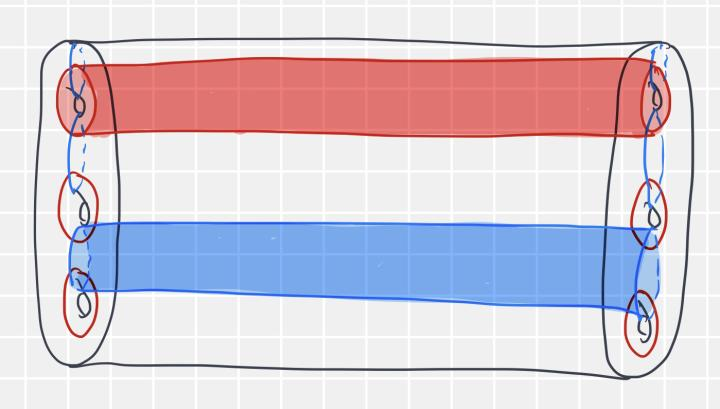
\includegraphics[width = 0.5\textwidth]{IMG_0627.jpg}
	 	\caption{(boring) mapping cylinders in \(M = F\times I\)}
	 \end{figure}

	 Suppose \(F\) has genus \(g\), then we can construct a system of essential simple closed curves \(k_1, \ldots, k_{2g}\) such that \(k_i\) and \(k_j\) intersect once traversely if \(i = j \pm 1\), and they are disjoint otherwise. If you have trouble finding such system, email me at \texttt{mujie.wang@bc.edu} for more assistance. For each \(k_j\), there is an cylinder \(G_j = k_j \times I\) embedded in \(M\). A pair of cylinders \(G_i\) and \(G_j\) intersect if and only if \(k_i\) and \(k_j\) intersect, and the intersection \(G_i \cap G_j\) is exactly \((k_i \cap k_j)\times I\).  

	 Here comes the second hardest part of this fake proof. 


\end{proof}

\end{document}